\Aufgabe[20]{Der Weg der Daten}{
    \begin{minipage}[t]{0.85\textwidth}
        \begin{enumerate}
            \item Öffnet im Browser Orinoco: \UrlAndCode{klassenkarte.de/oo/}
            \item Aus der linken Spalte benötigen wir die Elemente \emphColB{Eingabe, Funktion, Ausgabe und Datenfluss}.
            \item Wählt zwei verschiedene Formelfelder eurer Tabelle aus und erstellt ein Diagramm mit den genannten Elementen, das darstellt, welche Daten in die Berechnung einfließen, welche ausgegeben werden und was für eine Berechnung durchgeführt wird.
            \item Erstellt möglichst viele Diagramme auf verschiedenen Abstraktionsebenen.
        \end{enumerate}
        
        \vspace{0.2cm}
        \Loesung{
            Ein paar Beispiele für eine Zelle. Es gibt natürlich sehr viele Möglichkeiten.\\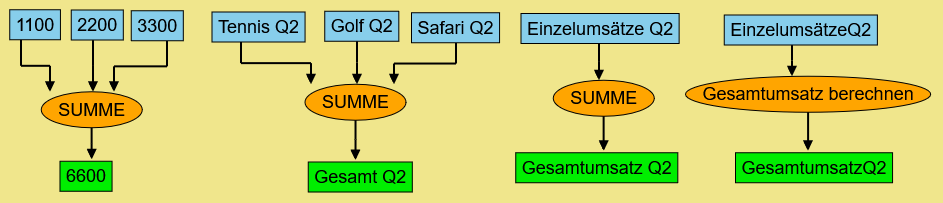
\includegraphics[width=\textwidth]{_Aufgaben/img/orinoo.png}
        }
    \end{minipage}
}
